\begin{fullwidth}
\chapter[Rainfall as a driver of epidemic cholera: Comparative assessments of the effect of intra-seasonal precipitation events]{Rainfall as a driver of epidemic cholera:\\Comparative assessments of the effect of\\intra-seasonal precipitation events}\label{ch:cholera-rainfall}
This section is adapted from:
\longfullcite{Lemaitre:RainfallDriverEpidemic:2019}.%\footnote[][-4\baselineskip]{JL, JP-S and DP developed the numerical tools required for the comparison. JL and DP conducted the numerical analyses for the deterministic model while JP-S conducted the numerical analyses for the stochastic model. AR and DP designed the framework for this study. JFW provided the epidemiological data. CS analyzed the data and prepared the model input. All authors contributed to the discussion of the results and writing of the manuscript.}.


\section{Résumé}

The correlation between cholera epidemics and climatic drivers, in particular seasonal tropical rainfall, has been studied in a variety of contexts. Several mechanistic models of cholera transmission have included rainfall as a driver by focusing on two possible transmission pathways: either by increasing exposure to contaminated water (e.g. due to worsening sanitary conditions during water excess), or water contamination by freshly excreted bacteria (e.g. due to washout of open-air defecation sites or overflows). In this chapter, the explanatory power of these different modeling structures is assessed by formal model comparison using deterministic and stochastic models of the type susceptible-infected-recovered-bacteria (SIRB). The incorporation of rainfall effects is generalized using a nonlinear function that can increase or decrease the relative importance of the large precipitation events. Our modelling framework is tested against the daily epidemiological data collected during the 2015 cholera outbreak within the urban context of Juba, South Sudan. This epidemic is characterized by a particular intra-seasonal double peak on the incidence in apparent relation with particularly strong rainfall events. Our results show that rainfall-based models in both their deterministic and stochastic formulations outperform models that do not account for rainfall. In fact, classical SIRB models are not able to reproduce the second epidemiological peak, thus suggesting that it was rainfall-driven. Moreover stronger support is found across model types for rainfall acting on increased exposure rather than on exacerbated water contamination. Although these results are context-specific, they stress the importance of a systematic and comprehensive appraisal of transmission pathways and their environmental forcings when embarking in the modelling of epidemic cholera.
\end{fullwidth}

\section{Rainfall and the transmission of cholera}\label{sec:rainfall-cholera-transmission}
Two main exposure pathways fuel cholera transmission across endemic and epidemic settings.
First, discovered by John Snow during the 1854 Broad Street cholera outbreak, an \textit{indirect} exposure occurs from consumption of water contaminated by untreated sewage\cite{Snow:ModeCommunicationCholera:1855}. Here, rainfall and the ensuing hydrologic transport processes might play a role in water contamination, for instance through the washout of open-air defecation sites and sewage circulation in the environment, which is thought to have started the Haitian 2010 outbreak\cite{Piarroux:UnderstandingCholeraEpidemic:2011}.
\textit{Direct}, or human-to-human exposure occurs when the bacteria is transmitted from an infected directly to a susceptible person, for example via contaminated food or fomite. In this case, environmental factors do not play a major role, except for transmission changes due to behaviour modifications.
The mechanism behind the spatio-temporal transmission dynamics of a cholera epidemics has been postulated to be a combination of environmentally-mediated and direct exposures\shortcite[-4\baselineskip]{Sugimoto:HouseholdTransmissionVibrio:2014,Bi:MicroscaleSpatialClustering:2016,Lessler:MeasuringSpatialDependence:2016,Rinaldo:ModelingKeyDrivers:2017}.
% Cholera and climate (STOP)
 \begin{marginfigure}[-2\baselineskip]
\centering
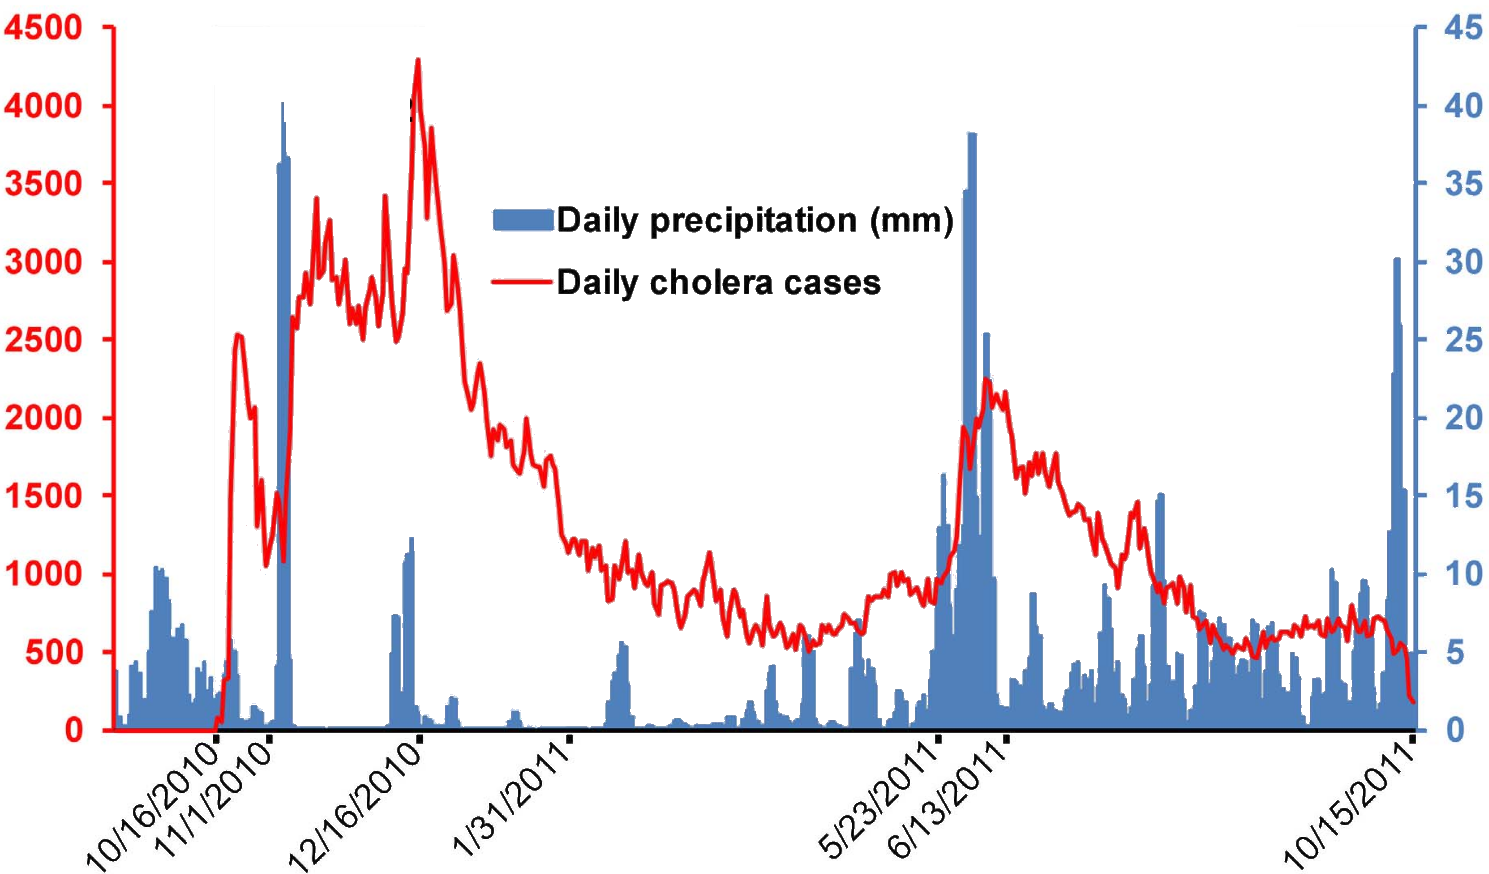
\includegraphics{fig/cholera-rainfall.png}
\margincaption[Daily cholera cases and rainfall in Haiti]{\footnotesize Daily cholera cases (red) and daily rainfall (blue) in Haiti from September 15, 2010 to October
16, 2011. A clear visual correlation between heavy rainfall event and case resurgence is observed. Adapted from \fullcite{Gaudart:SpatioTemporalDynamicsCholera:2013}.}
\label{rain}
\end{marginfigure}
\paragraph{Cholera and Rainfall} The relationship between different climatic and environmental factors and the transmission of cholera  has long been studied. Works linking cholera outbreaks to anomalies in the El Niño Southern Oscillation\shortcite{Colwell:GlobalClimateInfectious:1996, Pascual:CholeraDynamicsNinoSouthern:2000, Hashizume:DifferentialEffectIndian:2013}  have paved the way for a new field in epidemiological research. For large-scale infection patterns, many studies highlighted the role of climatic drivers on cholera dynamics, mostly focusing on climate change effects on disease spread\shortcite{Rinaldo:ModelingKeyDrivers:2017,Hashizume:EffectRainfallIncidence:2008,Magny:CholeraOutbreakSenegal:2012,Rodo:ClimateChangeInfectious:2013,Ramirez:NinoClimateCholera:2016,Vezzulli:ClimateInfluenceVibrio:2016, Rinaldo:ModelingKeyDrivers:2017} or on the impacts of spatial and temporal heterogeneities\shortcite{Reiner:HighlyLocalizedSensitivity:2012, Baker-Austin:EmergingVibrioRisk:2013, Vezzulli:OceanWarmingSpread:2013, Cash:CholeraShigellosisDifferent:2014,Escobar:GlobalMapSuitability:2015, Vezzulli:EffectsGlobalWarming:2015,Perez-Saez:ClimatedrivenEndemicCholera:2017}. While the effect of temperature on \textit{Vibrio} survival has been well described, mainly regarding bacterial biology and ecology in natural environments, that of rainfall remains to be fully elucidated, possibly due to the multiple ways in which it can influence transmission at the local and regional scales\shortcite{Rinaldo:Reassessment20102011:2012,Eisenberg:ExaminingRainfallCholera:2013,Baracchini:SeasonalityCholeraDynamics:2017}. Indeed, intense rainfall events have been shown to alter infection risk through a variety of potential mechanisms, including: flooding, leading to sewage contamination of water sources\shortcite{Ruiz-Moreno:CholeraSeasonalityMadras:2007, Hashizume:EffectRainfallIncidence:2008}; increased hydrologic transport-driven iron availability in environmental waters that enhances pathogen survival and the expression of toxins\shortcite{Lipp:EffectsGlobalClimate:2002,Faruque:SeasonalEpidemicsCholera:2005, Hill:ToxigenicVibrioCholerae:2011}; dry spells inducing persistent low water levels leading to increased use of unsafe water sources\shortcite{Rebaudet:EnvironmentalDeterminantsCholera:2013}; and crowding during strong flood events\shortcite{Reiner:HighlyLocalizedSensitivity:2012}.

Most countries where associations between rainfall and cholera risk have been studied experience endemic cholera transmission\shortcite{Rinaldo:ModelingKeyDrivers:2017}. Empirical studies have shown a range of correlations, both positive and negative, endowed with time lags ranging from weeks to months\shortcite{Ruiz-Moreno:CholeraSeasonalityMadras:2007,Emch:SeasonalityCholera1974:2008,Magny:CholeraOutbreakSenegal:2012}. In general, rainfall has been found to enhance cholera transmission, but there is evidence that propagation buffer effects in wet regions may be due to pathogen dilution\shortcite{Ruiz-Moreno:CholeraSeasonalityMadras:2007}. Such variability reflects the variety of potential mechanisms whereby rainfall may alter infection risk. Similarly, a clear empirical correlation between intense rainfall and enhanced transmission is found in several regions hit by cholera epidemics\shortcite{Magny:EnvironmentalSignaturesAssociated:2008,Rebaudet:EnvironmentalDeterminantsCholera:2013,Rebaudet:CholeraCoastalAfrica:2013,Jutla:WaterMarkerMonitored:2013,Gaudart:SpatioTemporalDynamicsCholera:2013}. The Haitian case, which has been in the midst of a major outbreak since October 2010\shortcite{Frerichs:NepaleseOriginCholera:2012,Gaudart:SpatioTemporalDynamicsCholera:2013,Kirpich:CholeraTransmissionOuest:2015,ERCCECHO:HaitiHurricaneMatthew:2016,Camacho:PredictionCholeraDynamics:2016,Pasetto:RealtimeProjectionsCholera:2017,Khan:AssessmentRiskCholera:2017}, has been studied under that angle, but its patterns have been argued to require a specific understanding\shortcite{Piarroux:UnderstandingCholeraEpidemic:2011}. Rainfall was therein is empirically associated with sudden resurgence of cholera infections via the analysis of reported cases\shortcite{Gaudart:SpatioTemporalDynamicsCholera:2013}, but a direct, causal relationship has only begun to be quantitatively examined\shortcite{Rinaldo:Reassessment20102011:2012,Eisenberg:ExaminingRainfallCholera:2013,Bertuzzo:ProbabilityExtinctionHaiti:2016}. Indeed, cholera case counts tend to rise sharply at the onset of seasonal heavy rains\shortcite{Adams:HaitiPreparesCholera:2012,Periago:EliminationCholeraTransmission:2012,Adams:CholeraHaitiTakes:2013}. Notably, for the Haitian outbreak, such nexus has been addressed theoretically\shortcite{Rinaldo:Reassessment20102011:2012,Eisenberg:ExaminingRainfallCholera:2013}. Results therein showed that at all spatial scales and locations examined, the tropical storms were correlated with increased cholera incidence with lags of the order of a few days. As a consequence, accounting for the related forcing of dynamic models resulted in improved fits of reported incidence. 

Properly incorporating the effects of rainfall in mathematical models of cholera transmission is thus paramount to discriminate among the above-mentioned alternative transmission pathways, thus unlocking a predictive framework to evaluate the potentially rainfall-sensitive efficacy of available intervention strategies in endemic and epidemic settings including vaccination, antibiotics, and improved access to water sanitation and hygiene (WaSH), leveraging the numerous solutions that exist for rainfall forecasting\shortcite{Rinaldo:Reassessment20102011:2012,Bertuzzo:ProbabilityExtinctionHaiti:2016}. This becomes  critically important when evaluating the number of averted infections by deploying vaccines, as was done in the aftermath of the passage of Hurricane Matthew\shortcite{Pasetto:RealtimeProjectionsCholera:2017}, or considering optimal deployment in space and time.

Rainfall has been accounted for in two main fashions in recent mathematical models of cholera. On one side, a contamination-centered approach suggesting that bursts of infections could be linked to increased contamination of the water compartment\shortcite{Rinaldo:Reassessment20102011:2012}. This process conceptualizes the washout of open-air defecation sites by hydrologic transport. The same `transport' effect may be realized by sewer collectors' overflows. In fact, both mechanisms have the net effect of charging progressively the bacterial concentration in the water reservoir\shortcite{Codeco:EndemicEpidemicDynamics:2001}. Pathogens' loads are washed out from a hydrologic catchment enclosing human settlements and their infective individuals shedding bacteria. Therein, pathogen survival and thus the toxicity of their loads depend on hydrologic residence time distributions\shortcite{Rinaldo:Reassessment20102011:2012,Rinaldo:ModelingKeyDrivers:2017}. Such loads increase as a function of rainfall, which acts as proxy of runoff volumes. The second approach is exposure-centered and employs a rainfall-dependent exposure rate subsuming both pathogen availability and the probability of the ingestion of contaminated water during wet spells\shortcite{Eisenberg:ExaminingRainfallCholera:2013}. Although both approaches are physically plausible, they have not been compared directly on the same datasets within a formal statistical framework, which would allow to highlight their respective merits and further recommendations for their use in different settings.

In this chapter, the explanatory power of these different types of rainfall-driven mechanistic models applied to a cholera outbreak in South Sudan is compared. The link between rainfall and cholera during the outbreak recorded in Juba in 2015, when an intra-seasonal peak of cholera cases was recorded possibly in correspondence to intense precipitation events is quantitatively examined. The analysis of the lagged relationship between rainfall rates and revamped cholera incidence is addressed via dynamical compartmental models considered both in deterministic and stochastic versions incorporating both direct (human-to-human) and indirect (water-to-human) disease transmission, and rainfall effects on both contamination and exposure.
\section{Case study: the 2015 cholera outbreak in Juba, South Sudan}\label{sec:data sets}
\begin{figure}\centering
  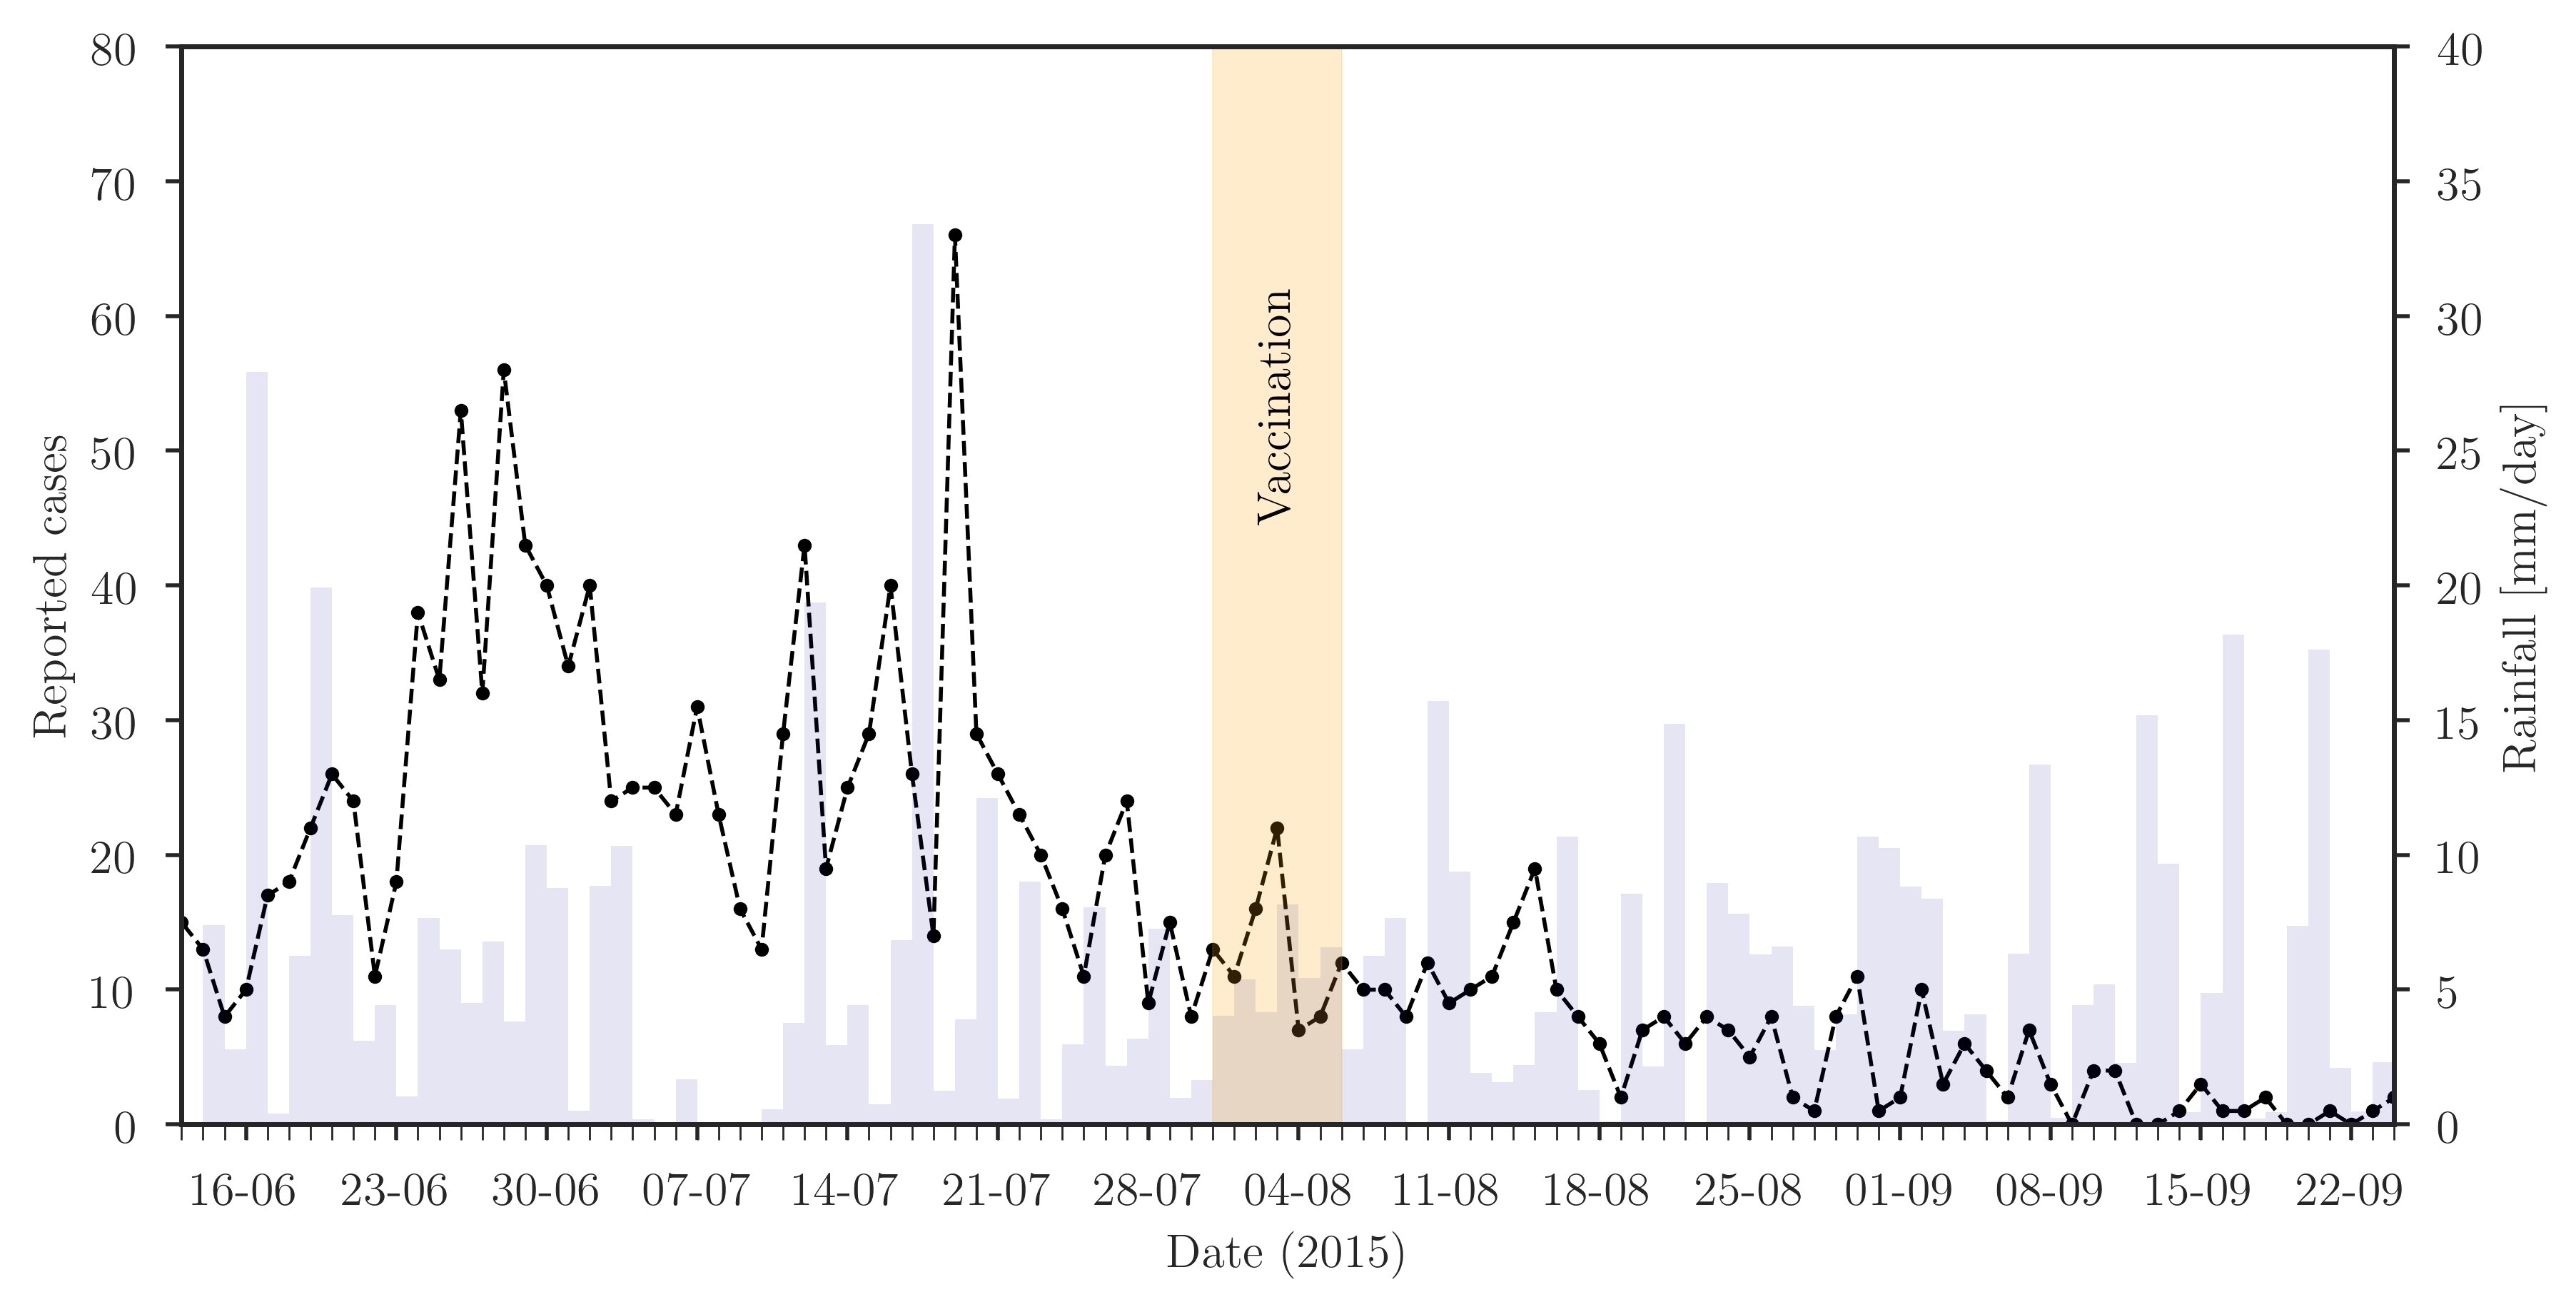
\includegraphics{fig_cholera-rainfall/Lemaitre_ACTROP_2018_42_R1_fig2.png}
  \caption[Cholera cases and precipitation during the 2015 epidemic in Juba][2\baselineskip]{Reported cholera cases (dots) and precipitation (bars) during the 2015 cholera epidemic in Juba. The timing of the vaccination campaign is highlighted in yellow.}\label{fig:report}
\end{figure}
In the past years, South Sudan had been struck by several cholera outbreaks\footnote{More details on the history of cholera in South Sudan are found in: \fullcite{Sciarra:MathematicalModelingCholera:2018}}. Here our analysis focuses on the 2015 outbreak in Juba, when a particular double peak of cholera cases occurred, probably associated to a strong intra-seasonal precipitation event (Figure~\ref{fig:report}). It uses epidemiological records for the 2014 and 2015 cholera epidemics that include cholera cases and hospitalization time series at the second-lowest administrative level  (Payams) as reported by the Ministry of Health of South Sudan. The recorded cases in the 7 Payams that constitute the administrative area of Juba have been aggregated to obtain the reported time series for the county level. The population data for Juba county is taken from the South Sudan National Bureau of Statistics\cite{SSNBS:PopulationProjectionsSouth:2015}.
These values were validated against the growth rate value stated by CIA\cite{CIA:SouthSudan:2015}. Daily rainfall estimates [mm d$^{-1}$] were obtained from the Climate Data Library (National Oceanic and Atmospheric Administration, NOAA)\cite{IRI/LDEO:ClimateDataLibrary:2016} for the years 2014 and 2015, with spatial resolution of {0.1}$^\circ$ (approximately $10$ km at the equator). The precipitation considered in the model have been spatially averaged over the study area. For what concerns the implementation of vaccines in 2015, 167'377 OCV doses were distributed in the county of Juba during 6 days of a mass vaccination campaign started in July 31, 2015\cite{Abubakar:FirstUseGlobal:2015,Azman:EffectivenessOneDose:2016,Parker:AdaptingGlobalShortage:2017}.
%FFN: South Sudan has a lot of one dose

\section{Cholera models}
\label{sec:meth}
The proposed model builds on the classic susceptible $S$, infected $I$, and recovered $R$ compartments for individuals, with an additional variable $B$ describing the concentration of the bacteria in the environment (thus, the model is named SIRB). Previous modelling exercises had considered rainfall intensity $J(t)$ either to i) multiplicatively increase water contamination with bacteria shed by infected  individuals\cite{Bertuzzo:ProbabilityExtinctionHaiti:2016,Pasetto:RealtimeProjectionsCholera:2017}, or ii) assumed that the rainfall multiplicatively increases the exposure to contaminated water\cite{Eisenberg:ExaminingRainfallCholera:2013}. Aiming at a systematic comparison of the effect of rainfall through these two different transmission pathways, a generalized formulation of these cholera-forced models, wherein both formulations are nested, is considered here.

Given the daily temporal resolution at which incidence data was available for the 2015 Juba's epidemic, a compartment of exposed individuals $E$ is introduced in addition to the S-I-R-B variables to describe the incubation period of the disease. This compartment is necessary to account the lag between the time of infection and the onset of the symptoms which result in reported cases. Moreover, in order to account for the vaccination campaigns that were deployed in Juba during August 2015, four compartments ($V^S$, $V^E$, $V^I$, and $V^R$) are added to describe the dynamics of vaccinated individuals and their removal from the pool of susceptibles.

The proposed generalized cholera model is described in fig.~\ref{diagram}, and formulated as:
\begingroup
\allowdisplaybreaks
\begin{eqnarray} \label{eq:fullmodel}
 \frac{dE}{dt} &=& \sigma F(t) S - (\phi + \mu +\nu) E \label{eq:E2}\\
 \frac{dI}{dt} &=& \phi E - (\gamma + \mu + \alpha) I \label{eq:I2}\\
 \frac{dR}{dt} &=& (1-\sigma) F(t) S + \gamma I - (\rho + \mu+\nu) R \label{eq:R2}\\
 \frac{dB}{dt} &=& - \mu_B B +\underbrace{\theta\left[1 + f_{\mathcal{C}}\left(J(t)\right) \right] (I+V^I)}_{\text{shedding}} \label{eq:B2}\\
\frac{dV^S}{dt} &=& \nu S - \mu V^S+ \rho_{v} V^R - (1-\eta) F(t) V^S \label{eq:VS2}\\
 \frac{dV^E}{dt} &=& \nu E + \sigma (1-\eta) F(t) V^S-(\phi + \mu) V^E \label{eq:VE2}\\
 \frac{dV^I}{dt} &=&  \phi V^E -(\gamma + \alpha + \mu) V^I \label{eq:VI2}\\
 \frac{dV^R}{dt} &=& \nu R -(\mu +\rho_{v})V^R +\gamma V^I +(1-\sigma) (1-\eta) F(t) V^S\label{eq:VR2}\; ,
\end{eqnarray}
\endgroup
where $F(t)$ takes into account both human-to-human transmission and nonlinear water-to-human transmission:
\begin{equation}
  F(t) = \beta_B \underbrace{ \left[\frac{B}{K + B} \right] \bigg(1+f_{\mathcal{E}}\left(J(t)\right)\bigg)}_{\text{indirect transmission}} + ~\beta_{I} \underbrace{\frac{(I+V^I)}{H}}_{\text{direct transmission}}.
\label{eq:force2}
\end{equation}

As few reliable data on changes in Juba's population are available for the years of interest (2014 and 2015), the total population $H$, is assumed to be constant, which implies that the number of susceptible individuals at time $t$ is $S(t) = H - I(t) - E(t) - R(t) - V^S(t) - V^E(t) - V^I(t) - V^R(t)$. Individuals are removed from the susceptible compartment $S$ at rate $F(t)$, becoming either symptomatically or asymptomatically infected with probabilities $\sigma$ and $(1-\sigma)$, respectively. Symptomatically infected, $I$, shed \textit{V.~cholerae} into the local watershed at rate $\theta$. 
The infectious period is governed by parameter $\gamma$, which determines the portion of infected individuals that enter the recovered compartment $R$, joining the asymptomatic infected. Recovered individuals return to the susceptible compartment at a rate $\rho$, describing the average rate of loss of immunity for individuals that previously had been asymptomatic or symptomatic infected. Parameters $\alpha$ and $\mu$ concern cholera related and unrelated death rates, respectively. The compartment $B$ quantifies the concentration of \textit{V. cholerae} in the local (conceptualized) water reservoir, which is used to estimate the probability of exposure to the contaminated water in (\ref{eq:force2}) through the term $\beta_B  \frac{B}{K+B}$, where  $\beta_B$ is the maximum exposure rate and $K$ is the half-saturation constant of the dose-response function of \textit{V.~cholerae}\cite{Codeco:EndemicEpidemicDynamics:2001}. Parameter $K$ is set to unity by considering the change of variable $\tilde{B}=B/K$. The parameter $\mu_B$ expresses the rate of decay of bacteria in the environment. 
Exposed individuals become symptomatic infected at a rate $\phi$, which corresponds to an average incubation period of $1/\phi\approx$ 1.5 days\cite{Azman:IncubationPeriodCholera:2013}.
Functions $f_{\mathcal{C}}\left(J(t)\right)$ and $f_{\mathcal{E}}\left(J(t)\right)$ account for the rainfall effect respectively by increasing the bacteria contamination in the water reservoir or directly through amplifying the exposure in the force of infection.
\begin{figure}
  \centering
  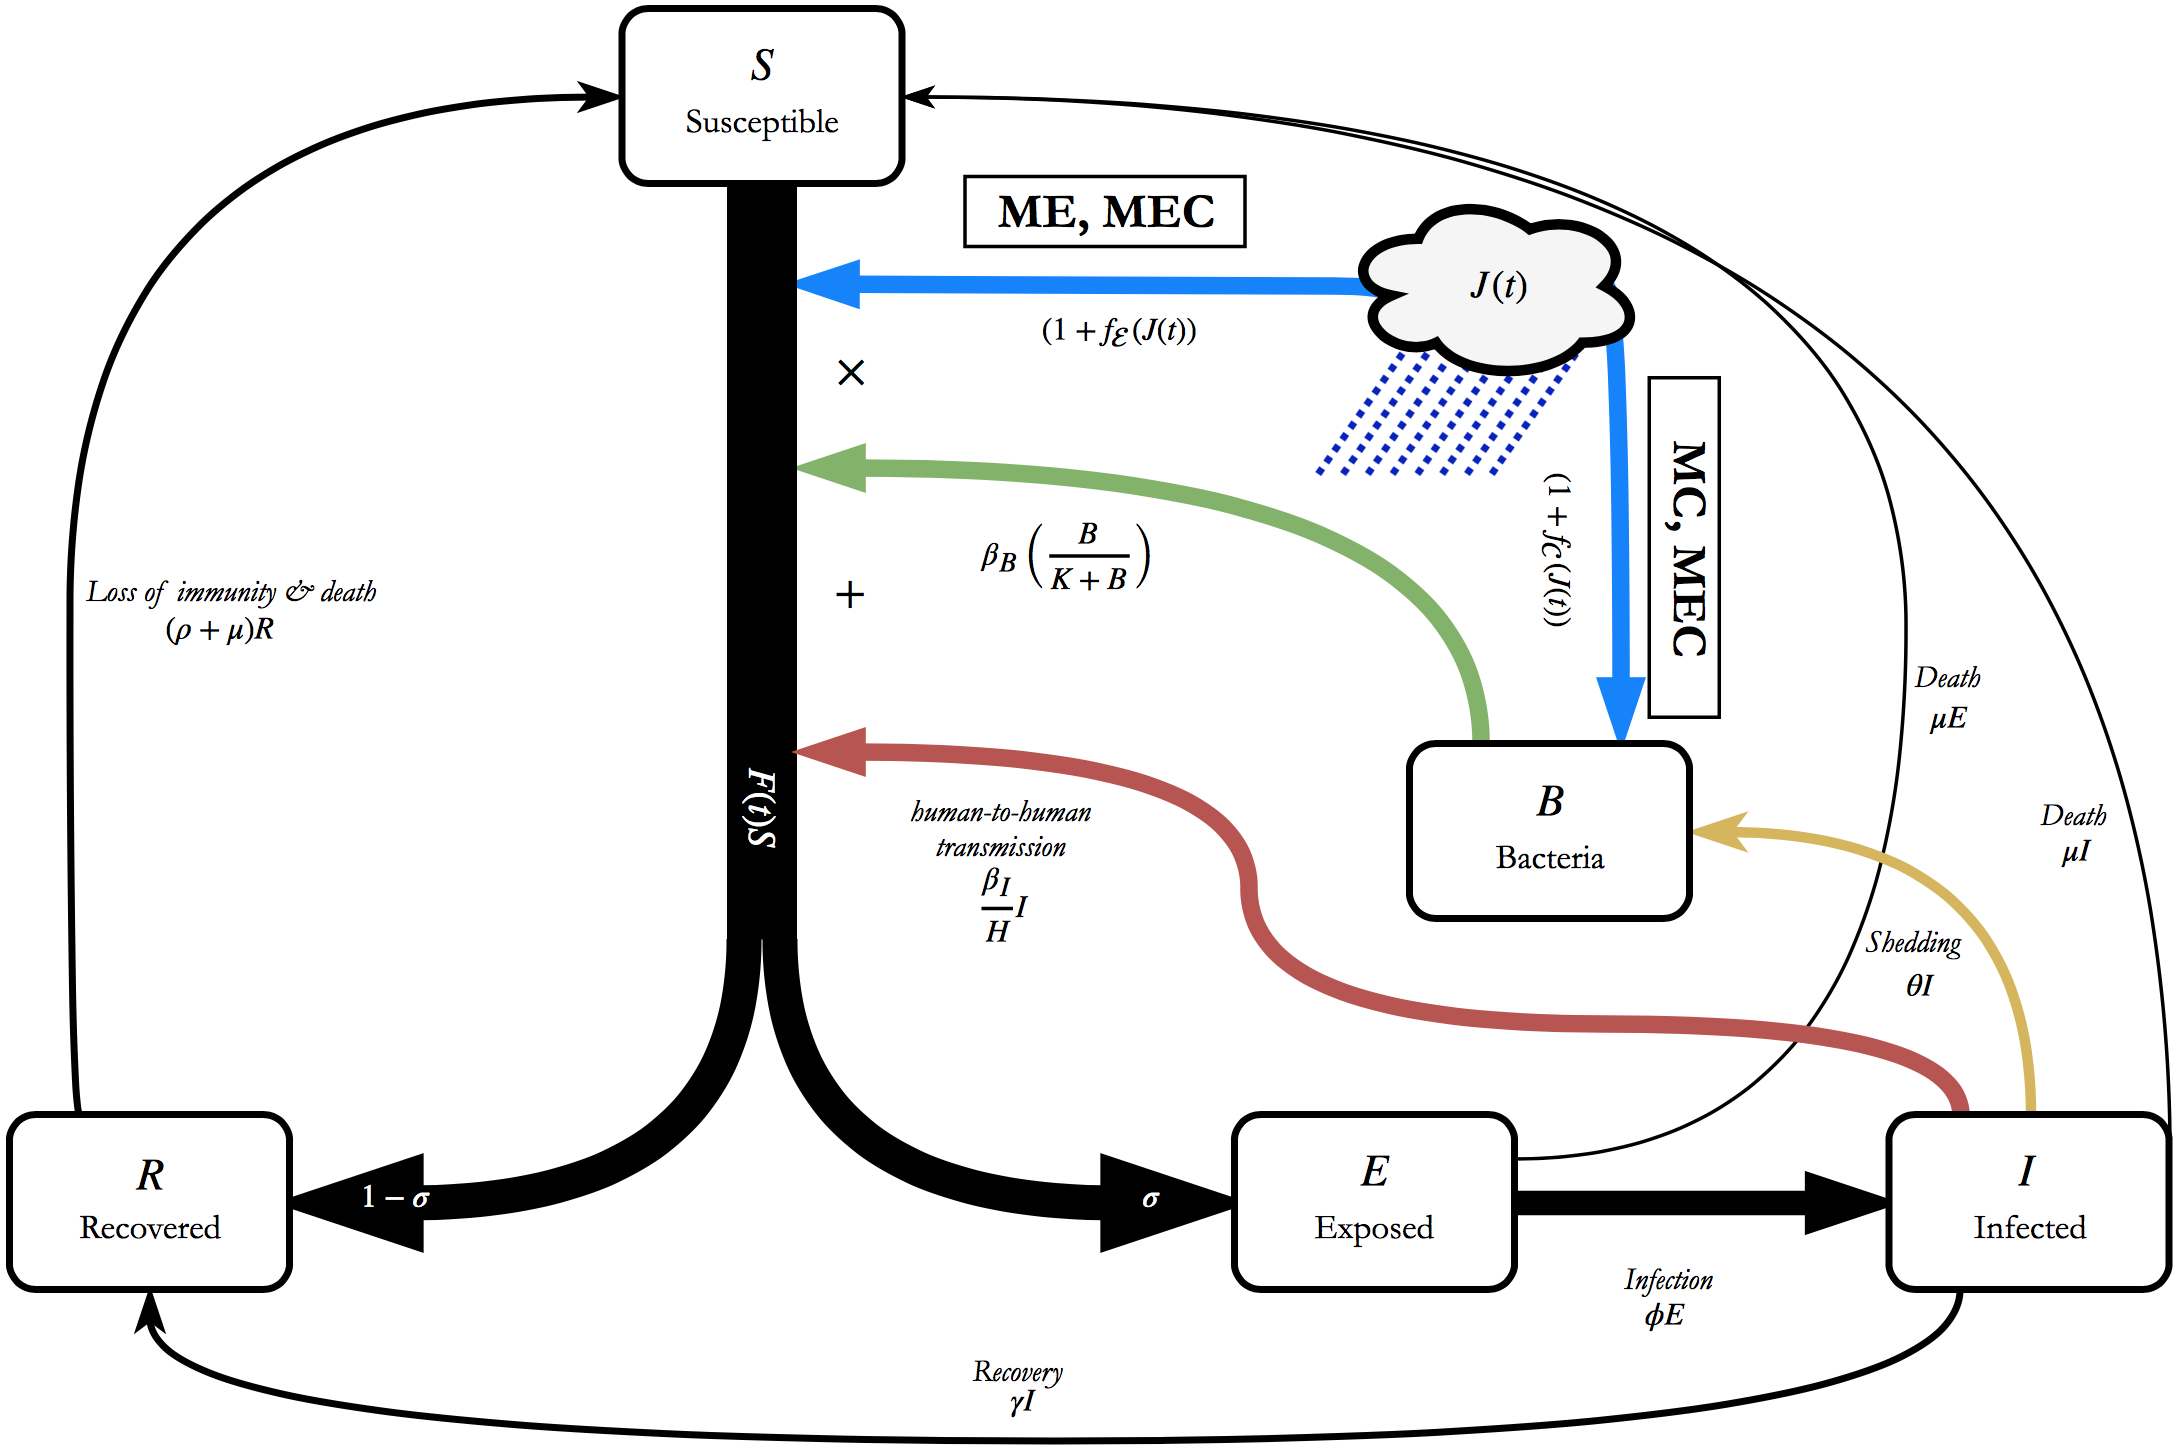
\includegraphics{fig_cholera-rainfall/Lemaitre_ACTROP_2018_42_R1_fig1.png}
  \caption[Transition diagram for the competing cholera models]{Transition diagram for the different cholera models considered, with the different variations \textsc{me}, \textsc{MR}, and \textsc{mec} indicated.}
  \label{diagram}
\end{figure}
With the objective of assessing the importance of rainfall on cholera transmission, a generalization of the linear relation found in the litterature\footnote{Specifically in the reference "exposure" model: \parencite{Eisenberg:ExaminingRainfallCholera:2013} and in the refered "contamination" model \parencite{Rinaldo:Reassessment20102011:2012}} by using a nonlinear function form for  $f_{\mathcal{C,E}}\left(J(t)\right)$, reading:
\begin{equation}
    f_{\mathcal{C,E}}\left(J(t)\right)=\lambda_{\mathcal{C,E}} \left(\frac{J(t)}{\max_t J(t)}\right)^{\alpha_{\mathcal{C,E}}}
    \label{eq:nonlinear_rain}
\end{equation}
\begin{marginfigure}
	\centering
	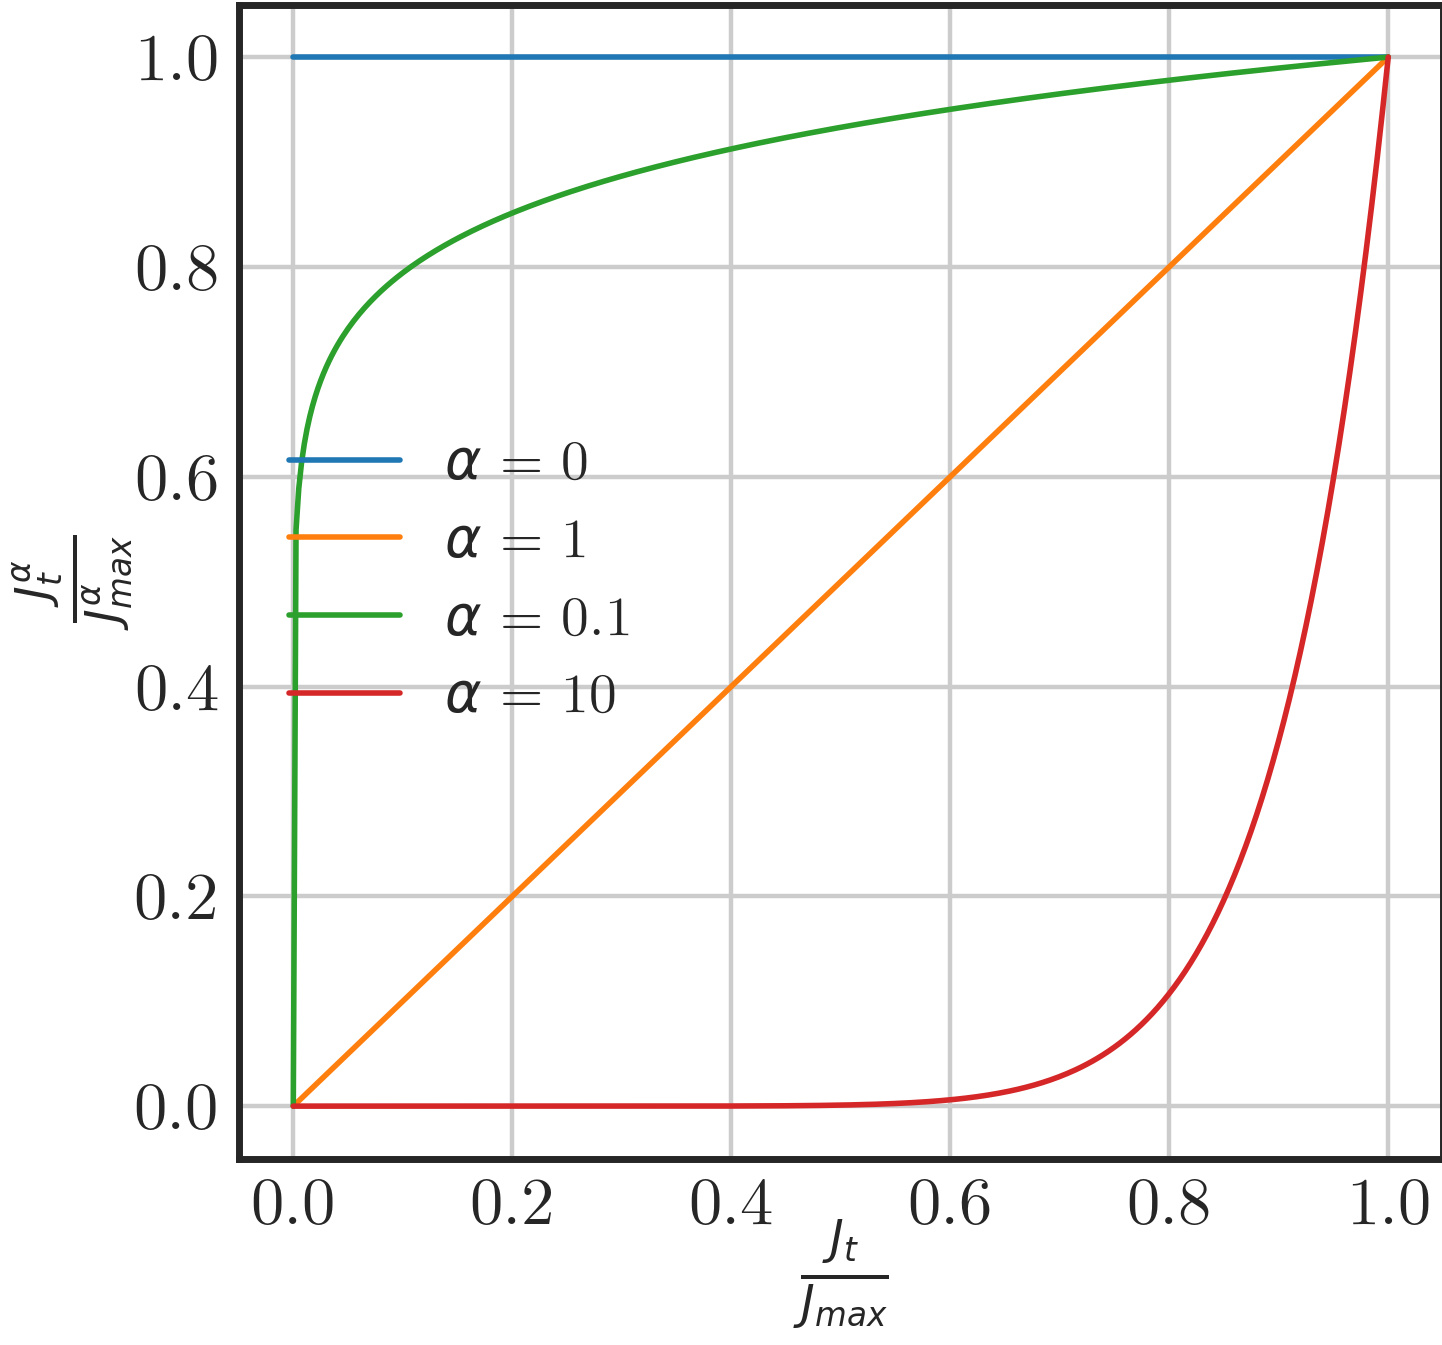
\includegraphics{fig_cholera-rainfall/alpha.png}
	\margincaption[Non-linear rainfall effect on transmission]{$\left(\frac{J_t}{J_{max}}\right)^\alpha$ for different values of $\alpha$. For $\alpha = 1$, the linear model described in previous works is obtained \parencite{Eisenberg:ExaminingRainfallCholera:2013, Rinaldo:Reassessment20102011:2012}. Larger $\alpha$ corresponds to an increased relative importance of heavy rainfall events.}
	\label{fig:alpha}
\end{marginfigure}
where the subscripts $_\mathcal{C,E}$ respectively denote the effect of rainfall on exposure and contamination, $\max_t J(t)$ is the maximum recorded rainfall intensity during the epidemic, and the $\alpha_{\mathcal{C,E}}\ge0$ controls for the relative importance of different rainfall intensities in their effect on the force of infection. Indeed, since the ratio $\frac{J(t)}{\max_t J(t)} \in [0,1]$, for $\alpha_{\mathcal{C,E}} \gg 1$ the ratio will tend to 0 for all small precipitation events, leaving only the effect of the strongest events, whereas for $\alpha_{\mathcal{C,E}} < 1$ all precipitation events will be assigned a similar weight in the force of infection. Note that by setting $\alpha_{\mathcal{C,E}} = 1$, the formulations found in litterature is recovered. The flexibility allowed by (\ref{eq:nonlinear_rain}) is therefore able to discriminate between rainfall effects along a continuum from acting on disease transmission regardless of intensity to a threshold-like effect for the largest events which could be associated to severe flooding causing damages to the city's water and sanitary system, for instance leading to sewer overflow.
\marginnote[3\baselineskip]{Note that in (\ref{eq:force2}) precipitation enters in the term $\left(1+f_E \left(J(t)\right)\right)$ which entails water-to-human transmission also when $J(t)=0$ differently from what happens in the refered exposure model fom \fullcite{Eisenberg:ExaminingRainfallCholera:2013}.}.

During the vaccination campaign, oral cholera vaccines (OCV) doses are assumed to be distributed with equal rate $\nu$ to susceptible, exposed and recovered individuals, which enter the compartments $V^S$, $V^E$ and $V^R$. As the OCV provides only a partial immunity having efficacy $\eta$, $0\leq \eta \leq 1$, vaccinated susceptibles ($V^S$) can become exposed ($V^E$) through a decreased force of infection of a factor $(1-\eta)$ with respect to non-vaccinated individuals. Vaccinated infected individuals behave exactly like infected ones, but are placed in a different compartment to exclude them from future vaccination campaigns. After recovering at  rate $\gamma$, they lose their vaccine protection at rate $\rho_{v}$.


\subsection{Competing models}
The relevance of the two rainfall-driven transmission pathways is assesed here by comparing the impact the results of the following models:
\begin{itemize}
 \item \textsc{mn} SIRB model without rainfall: $\lambda_{\mathcal{C}} = \lambda_{\mathcal{E}} = 0$, $\beta_{I} = 0$, as the null hypothesis for the importance of rainfall.
  \item \textsc{mc} SIRB model where for rainfall enhances the \textit{contamination} of the water reservoir: $\lambda_{\mathcal{E}} = 0$, $\beta_{I} = 0$. 
  \item \textsc{me} SIRB model where rainfall increases the \textit{exposure} to bacteria: $\lambda_{\mathcal{C}} = 0$, $\beta_{I} = 0$. 
  \item \textsc{mec} SIRB model combining both approaches \textsc{mc} and \textsc{me} ($\beta_{I} = 0$). Both ways of accounting rainfall play a role simultaneously.
\end{itemize}
\marginnote[-5\baselineskip]{\textsc{me} models uses a similar transmission pathway as in \textcite{Eisenberg:ExaminingRainfallCholera:2013}, whereas \textsc{mc} models were described in \textcite{Rinaldo:Reassessment20102011:2012}}
\begin{table}[h!]
\centering
\begin{tabular}{lccccc}
\toprule
     Model       & $\lambda_{\mathcal{C}}$ & $\alpha_\mathcal{C}$ & $\lambda_{\mathcal{E}}$ & $\alpha_\mathcal{E}$ & $\beta_I$   \\
    \hline
    \textsc{mn} &       -    &    -   &       -      &       -      &  - \\
    \textsc{mnh} &     -      &   -    &    -         &        -     &   X\\
    \textsc{mc} &       X   &   X   &     -        &       -      &  - \\
    \textsc{me} &         -  &   -    &       X     &    X         & -  \\
    \textsc{mch}&       X   &   X   &      -       &     -        & X  \\
    \textsc{meh}&        -   &  -     &       X     &    X         & X  \\
    \textsc{mec}&       X  &   X   &       X     &     X       & -\\
    \textsc{mech}&       X  &   X   &       X     &     X        &   X\\
\bottomrule
\end{tabular}
\caption[Parameters considered in the eight compared models.]{Parameters considered in the eight compared models.  $\lambda$ and $\alpha$ characterize the functional forms considering the precipitation (eqn.~\ref{eq:nonlinear_rain}). $\beta_I$ is the exposure for human-to-human transmission.}
\label{tab:models}
\end{table}
 For each model is explored the possibility of adding explicitly direct, human-to-human transmission ($\beta_{I} > 0$), which is indicated with an \textsc{H} at the end of the model name: \textsc{mnh}, \textsc{mch}, \textsc{meh}, and \textsc{mech}. Table~\ref{tab:models} summarizes the different parameters associated with the considered models.

 The eight models are compared on the basis of their ability to match the time series of daily reported cases during the cholera epidemic in Juba of 2015. Table S.1 summarizes which parameters are calibrated for each model and their prior distribution. The degrees of freedom of the models, $n_p$, vary from $n_p=7$ for \textsc{mn} to $n_p=12$ for \textsc{mech}. Given the low number of daily reported cases and their ensuing variability, a stochastic equivalent is also implemented\footnote[][-10\baselineskip]{The sole difference in formulation is the introduction of overdispertion in the infection process. The force of infection is multiplied by a time-continuous white noise process \(\xi(t)\) defined as the differentiation of an integrated noise process \(\xi(t) = \frac{d}{dt}\Gamma(t)\), here taken to be a Gamma with mean \(\Delta t\) and variance \(\sigma^2 \Delta t\) : \[
\Gamma (t+\Delta t) - \Gamma (t) \sim \text{Gamma}\left( \frac{\Delta t}{\sigma^2}, \sigma^2\right). \]
Since \(\xi(t)\) is non-negative it can serve as a multiplicative noise onthe force of infection: \[ F^{stoch}(t) = F(t) \xi(t). \]This methods has been proposed in \fullcite{Breto:CompoundMarkovCounting:2011}.} of the deterministic ODE system (\ref{eq:fullmodel}-\ref{eq:VR2}) formulated as a continuous time partially observed Markov process model, accounting for both demographic and disease transmission stochasticities\cite{Breto:TimeSeriesAnalysis:2009}. 

\subsection{Models calibration}
\paragraph{Initial conditions} The past history of cholera epidemics in South Sudan, and particularly in Juba, plays an important role in the determination of the size of susceptible and recovered compartments at the beginning of the 2015 epidemic. These two compartments are also largely impacted by the rate of immunity loss, $\rho$, of the recovered individuals, which determines the duration of the stay in the $R$ compartment (from few months to several years), and the probability of asymptomatic infected, $1-\sigma$, which determines how many asymptomatics enter the $R$ compartment \footnote{values in literature range between $\sigma=0.5$, meaning one asymptomatic per each symptomatic infected, to less than $\sigma=0.01$, corresponding to more than 99 asymptomatic infected per each symptomatic infected\parencite{Fung:CholeraTransmissionDynamic:2014}}. The initial conditions must therefore be estimated for each parameter set considered during calibration.
\marginnote[-11\baselineskip]{For details about calibrated parameters and posterior distribution, the reader is referred to the supplemental information of \fullcite{Lemaitre:RainfallDriverEpidemic:2019}.}
 
 To take into account the uncertainty associated with the past epidemics and vaccination campaigns, the initial number of temporary immune individuals, $R_0$, in April 2014 is calibrated for each model.
 
 The detailed daily data of suspected cases during 2014 is used to estimate the associated number of recovered individuals. These undergo an exponential decay with average time of immunity loss $1/\rho$ (similarly to what done in\cite{Pasetto:RealtimeProjectionsCholera:2017}), thus obtaining a consistent estimate of the recovered in June 2016. Simulations are then initialized on the 5$^{th}$ of June 2015 considering two exposed individuals, two infected, and the associated steady-state bacteria concentration. 
 
\paragraph{Calibration} Calibration of the deterministic model is performed using a Markov Chain Monte Carlo (\textsc{mcmc})-based algorithm\footnote{Differential Evolution Adaptive Metropolis, \textsc{dream}: \parencite{Vrugt:MarkovChainMonte:2016}, which was developed to explore high-dimensional parameter spaces. Given the parameters' prior distribution, \textsc{dream} searches and selects new samples in the posterior distribution by using multiple \textsc{mcmc} chains that run in parallel and that jointly contribute to the computation of the proposal parameter samples. \textsc{Mcmc} chains  converge toward the posterior probability distribution based on the ho likelihood function of the data given the model output.} , which draws samples from the posterior distribution of the parameters.
Inference on the stochastic model is performed using a frequentist multiple iterated filtering algorithm\footnote{using a multiple iterated filtering (MIF) algorithm proposed by \parencite{Ionides:InferenceDynamicLatent:2015}, which is a frequentest-based approach for identifying the MLE that has proved successful even for a range of complex models of cholera dynamics \parencite{King:InapparentInfectionsCholera:2008,Baracchini:SeasonalityCholeraDynamics:2017}. The MIF2 algorithm, which employs iterated Bayes maps in the \texttt{pomp} package in R \parencite{King:StatisticalInferencePartially:2015} is configured using 120 initial parameter vectors for each model, built using Sobol sequences over the parameter bounds.}. Both model were fit against the daily reported cases accounting for over- or under- reporting, and assuming a Poisson distribution\shortcite{Camacho:CholeraEpidemicYemen:2018}. Each datapoint at reporting date $t_i$,  $y_{t_i}$, is assumed to belong to a Poisson distribution centered on the predicted infected incidence $C_i$\footnote{$ C_{t_i} = \int_{t_i}^{t_{i+1}} \phi \left(E(t) + V^E(t)\right) dt  $ for the deterministic model, and $ C_{t_i} = [N_{EI}(t_{i+1}) - N_{EI}(t_i)] + [N_{V^EV^I}(t_{i+1}) - N_{V^EV^I}(t_i)] $, where $N_{AB}$ denotes the stochastic counting process of transitions between classes $A$ and $B$ for the stochastic model} produced by a model and its associated parameter vector $\boldsymbol{\theta}$ altered by the reporting rate $\epsilon$, as:
\begin{equation}
 y_{t_i}  \sim \text{Poisson}\left(\epsilon \,C_{t_i}(\boldsymbol{\theta})\right), \; \epsilon > 0,
 \label{eq:obs}
\end{equation}
 Models were then compared using the Bayesian Information criterion (BIC), Bayes factors, and the likelihood ratio test for the nested models.
 
 
\section{Results}

\subsection{Selection of rainfall effects on transmission pathways}
The summary statistics of the deterministic and stochastic models considered in the study are given in Table~\ref{tab:stats}. Overall, the stochastic models outperform their deterministic counterparts for all model structures by $\approx 40$ log-likelihood units. Both model types agree in the significance of rainfall in explaining the time series of daily reported cases, in particular through the increased exposure pathway, although the specific ordering of the models differs between model types. Indeed, the BFs for the deterministic models suggest a strong support for model \textsc{mec}, followed by model \textsc{me} ($BF^{-1}_{ME,MEH} = 0.16$), with very little support for all other models ($BF^{-1}_{\boldsymbol{\cdot},MEH}< 10^{-2}$ for all other models than ME). For the stochastic model, the BFs estimated with the BIC suggest the strongest support for model \textsc{me}, with the basic SIRB model coming in second with 5 times less evidence ($BF^{-1}_{MN,ME} \approx 0.15$). 
\begin{table}[h!]
\centering
\small
\begin{tabular}{lcccccccc}
  \toprule
  & \multicolumn{4}{c}{Deterministic} & \multicolumn{4}{c}{Stochastic} \\
    \cmidrule(rl){2-5}\cmidrule(rl){6-9}
  Model & $n$ & $\hat{\ell}$ & BIC & ${BF}^{-1}$ & $n$ & \makecell{$\hat{\ell}$ \vspace{-.1cm} \\ \scriptsize{(s.e.)}}  & BIC  & $BF^{-1}$ \\ 
  \cmidrule(rl){2-5}\cmidrule(rl){6-9}
  \textsc{mn} &   7 & -368.62 & 770.27 & 3.1E-05 &   8 & \makecell{-326.45 \vspace{-.1cm} \\ \scriptsize{(0.105)}} & 690.65 & 1.5E-01 \\ 
   \textsc{mnh} &   8 & -368.95 & 775.64 & 1.1E-09 &   9 & \makecell{-327.52\vspace{-.1cm} \\ \scriptsize{(0.052)}} & 697.51 & 4.7E-03 \\ 
   \textsc{mc} &   9 & -358.32 & 759.11 & 5.5E-03 &  10 & \makecell{-323.50\vspace{-.1cm} \\ \scriptsize{(0.037)}} & 696.01 & 2.5E-02 \\ 
   \textsc{mch} &  10 & -359.06 & 765.30 & 1.7E-04 &  11 & \makecell{-324.89\vspace{-.1cm} \\ \scriptsize{(0.041)}} & 701.68 & 5.9E-04 \\ 
   \textsc{me} &   9 & -356.96 & \textsc{756.40} & 1.6E-01 &  10 & \makecell{\textsc{-319.81}\vspace{-.1cm} \\ \scriptsize{(0.035)}} & \textsc{687.38} & \textsc{1} \\ 
   \textsc{meh} &  10 & -358.06 & 763.30 & 6.3E-04 &  11 & \makecell{-320.64\vspace{-.1cm} \\ \scriptsize{(0.030)}} & 693.18 & 4.1E-02 \\ 
   \textsc{mec} &  11 & \textsc{-356.87} & 765.64 & \textsc{1} &  12 & \makecell{-320.17\vspace{-.1cm} \\ \scriptsize{(0.031)}} & 696.96 & 6.2E-03 \\ 
   \textsc{mech} &  12 & -357.55 & 771.73 & 2.4E-06 &  13 & \makecell{-320.38\vspace{-.1cm} \\ \scriptsize{(0.024)}} & 702.09 & 4.8E-04 \\ 
   \bottomrule
\end{tabular}
\caption[Model comparison statistics.]{Model comparison statistics. For each model is reported its number of parameters $n$, the associated estimated log-likelihood $\hat{\ell}$ (and its Monte Carlo standard error for the stochastic model), and the inverse of the Bayes Factor ($BF^{-1}$) with respect to the model with the largest evidence. The BFs for the deterministic models were computed directly from the parameters posteriors, whereas for the stochastic models they were estimated with the Bayesian Information Criterion (BIC) as $BF_{i} \approx e^{\frac{1}{2} \left( BIC_i - BIC_{min}\right)}$. The BIC for the deterministic models was computed using the maximum log-likelihood value visited with the MCMC algorithm across chains. Best values in each column are indicated in bold.}\label{tab:stats}
\end{table}
When considering only the BIC, model \textsc{me} ranks first for both the deterministic and the stochastic formulations. Interestingly, all models that include human-to-human transmission present smaller or equal log-likelihoods than their counterparts with only the bacteria compartment, which suggests that the data does not support both environmental and human-to-human transmission within the set of the models considered here.
\begin{figure*}
    \centering
    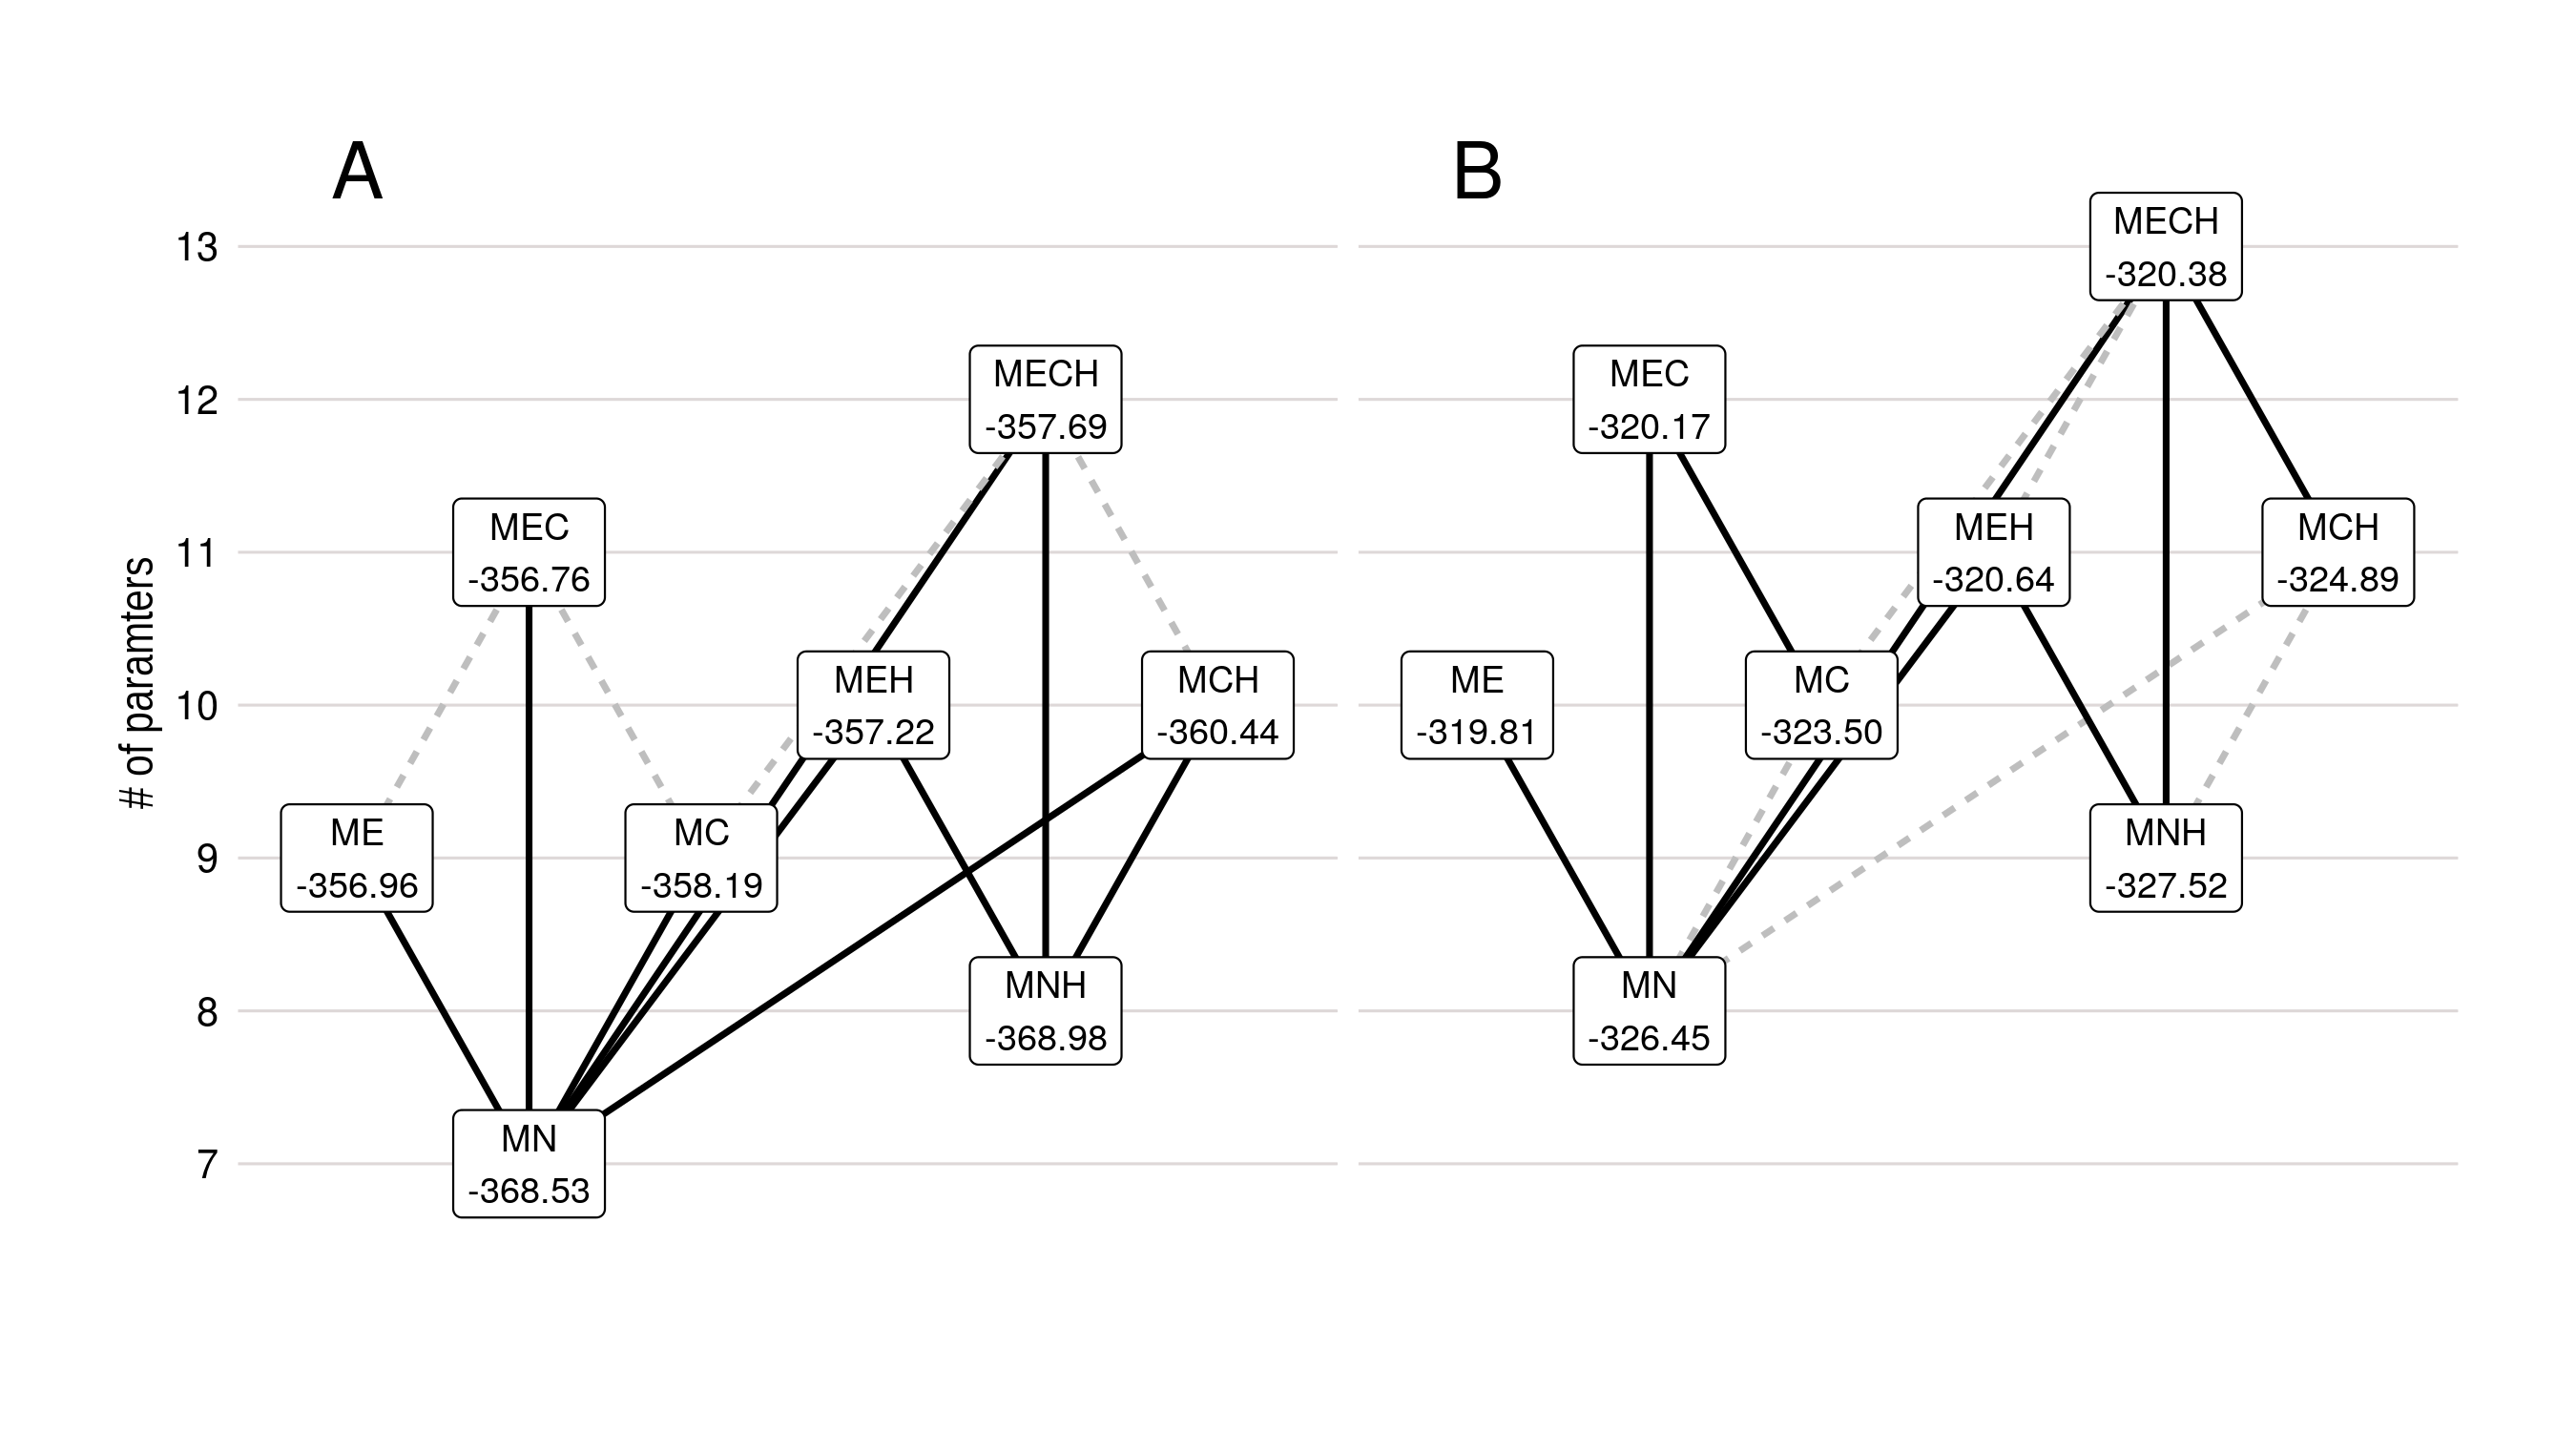
\includegraphics[width = \textwidth, trim = 11mm 19mm 10mm 12mm, clip]{fig_cholera-rainfall/Lemaitre_ACTROP_2018_42_R1_fig3.png}
    \caption[Likelihood ratio tests of model nesting]{Likelihood ratio tests of model nesting. The LL-tests were computed for each nested pair of models $\{\mathcal{M}_0, \mathcal{M}_1\}$, with parameter vectors $\boldsymbol{\theta}^0,\boldsymbol{\theta}^1$, for which at least on of the parameters that is not null is $\boldsymbol{\theta}^1$ is equal to 0 in $\boldsymbol{\theta}^0$. Each model is labeled with its associated estimated maximum log-likelihood value, $\hat{\ell}$, for the deterministic (A) and the stochastic (B) models, and linked based on whether the likelihood ratio is significantly (full black lines) or not (dashed gray lines) at the 5\% level. The absence of lines indicates a lower $\hat{\ell}$ for the more complex model.} 
    \label{fig:lltests}
\end{figure*}

The results of the nested LR-tests confirm the statistical significance of including rainfall in the cholera transmission models, with the effect on exposure better supported by the data in both model types than the effect on contamination. In the deterministic case, the extension of the basic SIRB (model \textsc{mn}) with rainfall effects were significant for all direct comparisons (Fig.~\ref{fig:lltests}~A). The addition of human-to-human transmission was not significant mostly due to the above-mentioned lower estimate of the log-likelihood in these models. When considering only a single effect of rainfall (either increasing exposure or contamination), \textsc{me} outperforms \textsc{mc} in terms of likelihood for the same number of parameters. Interestingly, the inclusion of rainfall-induced contamination in model \textsc{me} is rejected due to the very limited increase of the estimated log-likelihood of \textsc{mec}, in contrast with the BFs favouring the latter. Model \textsc{me} is thus the one retained by the LR-tests in the deterministic set of models. In the case of the stochastic models, the LR-tests also highlight the importance of the effect of rainfall on exposure rather than on contamination (Fig.~\ref{fig:lltests}~B). In fact, the much stronger performance of \textsc{mn} in comparison with its deterministic counterpart relative to all other model structures imposes a stronger condition for retaining additional transmission processes. Indeed, both models \textsc{mc} and \textsc{mch} were rejected when compared to \textsc{mn}, thus only models with rainfall-driven exposure were retained. As in the deterministic case, model \textsc{me} is the one finally retained due to the lack of significance of the inclusion of additional transmission processes. Note that the conclusion based on the LR-tests for the deterministic models should be taken with caution because the \textsc{mcmc} algorithm used for calibration does not directly aim at maximizing the likelihood, but rather at sampling from the posterior distribution of the parameters given the data and the model. Moreover, the best likelihood visited by the chains when sampling the posteriors that are used in the LR-tests is not a formal estimate of the models' likelihood. However, the fact that the LR-tests applied to both model types agree with the selection of \textsc{me} supports their use in both cases.


Both statistical methods for model comparison therefore agree about the importance of the effect of intra-seasonal rainfall on the exposure to transmission during the 2015 cholera epidemic in Juba. For the deterministic type of models the BFs suggest a stronger support for model \textsc{mec}, and the LR-tests for \textsc{me}, whereas for the stochastic models both the BIC-based estimates of BFs and the LR-tests favor \textsc{me}. 

\subsection{Intra-seasonal rainfall events and the 2015 Juba epidemic}

The comparison between the estimated output cases computed by the basic SIRB model (\textsc{mn}) and the most significant rainfall-based processes (\textsc{mec} and \textsc{me} for the deterministic and stochastic types, respectively) highlight the importance of rainfall in retrieving the second epidemiological peak (Figure~\ref{fig:sim}). Both deterministic and stochastic SIRB fit well the general trend of the data, but they clearly underestimate the large number of reported cases on the 19th of July (65 cases). Instead, the more complex models \textsc{me} and \textsc{mec} follow the SIRB dynamics and then are forced by the precipitation occurred in the 18th of July (33 mm/d)  toward the epidemiological peak. 
%
\begin{figure}[ht]
    \centering
    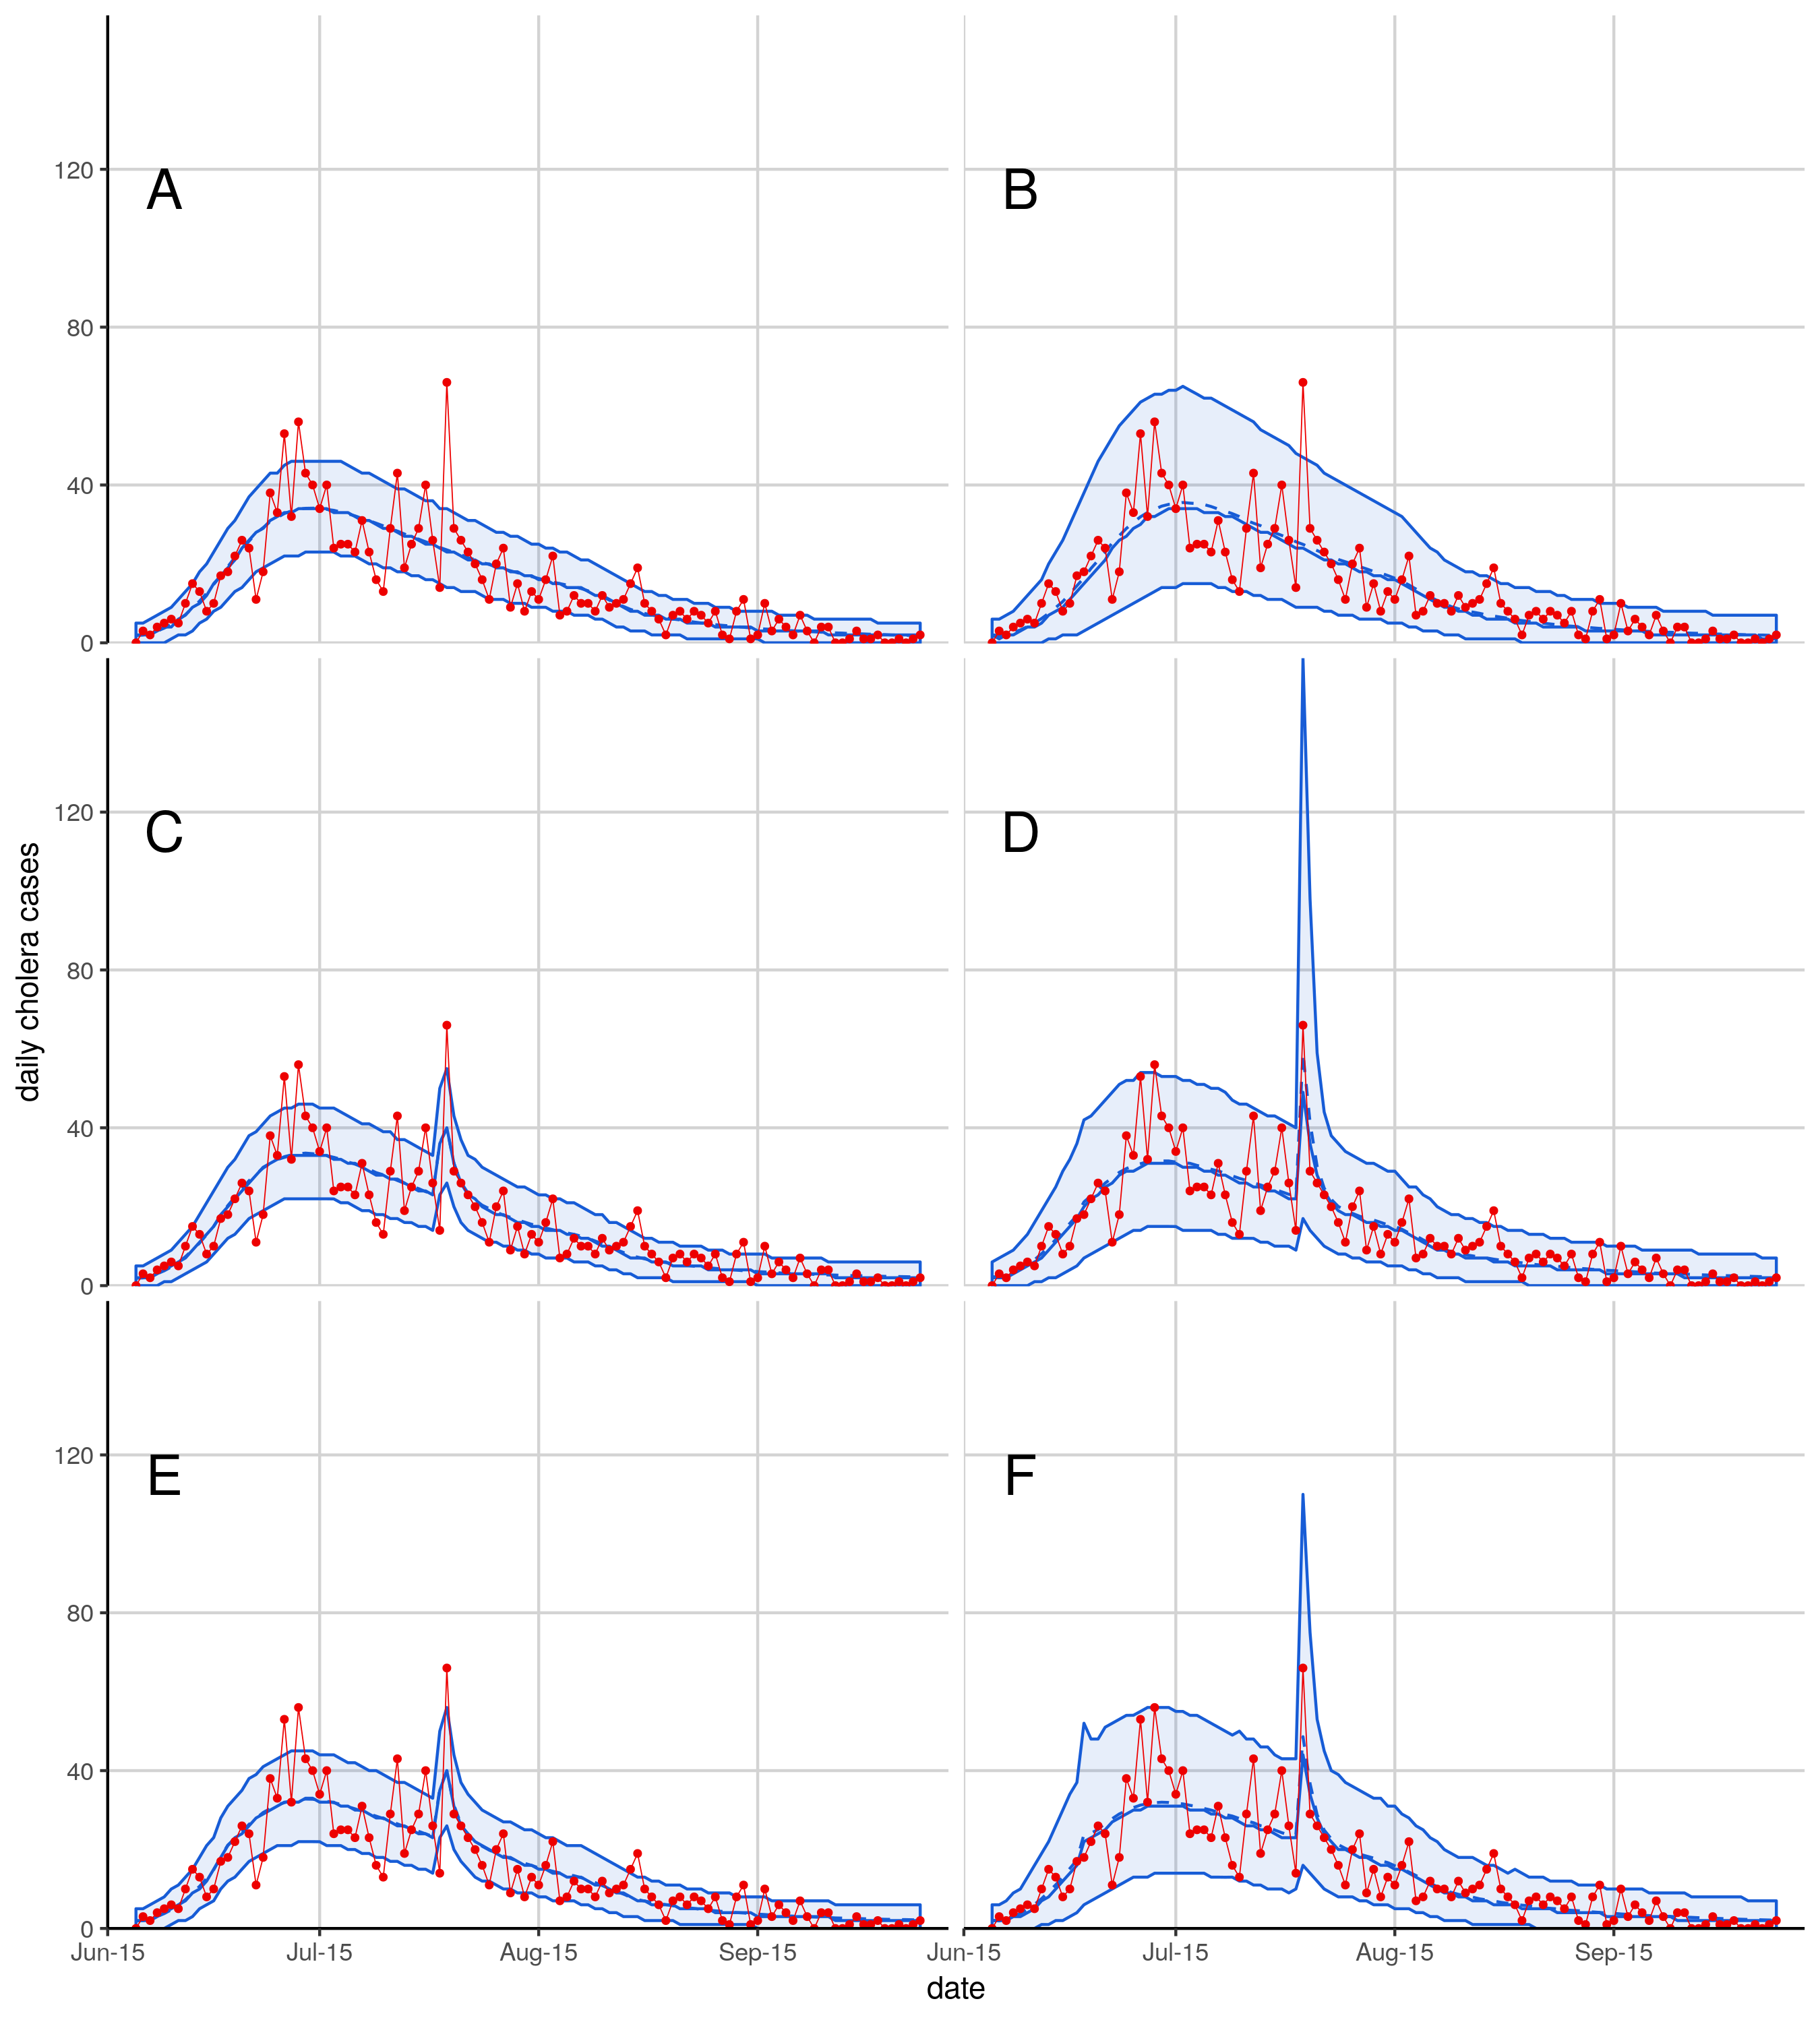
\includegraphics{fig_cholera-rainfall/Lemaitre_ACTROP_2018_42_R1_fig4.png}
    \caption[Fit of the different models]{Simulations of the \textsc{mn} (A-B), \textsc{me} (C-D) and \textsc{mec} (E-F) models. Simulations for the deterministic versions (A,C,E) are given by the mean (blue dashed line), median (blue full line) and 95\% simulation envelops (blue ribbon) of 100 simulations of the measurement model for each trajectory from 100 samples from the posteriors of model parameters against reported daily cholera cases (red line and dots). Simulations from the stochastic models (B, D, F) are given for 10'000 simulations of the stochastic process and measurement models.}
    \label{fig:sim}
\end{figure}

Model calibration results suggest that precipitations with smaller intensities did not have a strong impact on cholera transmission during the 2015 epidemic in Juba. Indeed, the exponents $\alpha_{\mathcal{C}}$ and $\alpha_{\mathcal{E}}$ were found to be systematically larger than 1. %  (as shown by posteriors of the deterministic models in fig. S.2 and the Monte Carlo confidence intervals for the stochastic \textsc{me} in fig. S.4 of the SI) --> appendix or not ? DECISION
  Thus, in the considered epidemic, the nonlinear function used to account for rainfall in the model (eqn.~\ref{eq:nonlinear_rain}) helps isolating the contribution of the largest rainfall.

The best measures of fit computed for the stochastic \textsc{me} (see Table~\ref{tab:stats}) are thus explained by a larger sensitivity to precipitation, which causes the match between the mean of the simulated cases and the data during the second peak.

Comparing the two model types, stochastic results have a larger 95\% confidence interval, which better encompass most of the data. In particular, both epidemiological peaks are well captured by the stochastic models, while the deterministic results systematically underestimate them. Two factors contribute to this result: the intrinsic stochastic nature of the model, that requires the simulation of various model runs for the same set of parameters, and the noise that necessarily perturbs the force of the infection yielding an overdispersion in infections. The standard deviation of such (assumed white) noise is estimated in each stochastic model, and it is interesting to note that the MLE obtained for \textsc{ME} is slightly smaller than in \textsc{MN} (0.028 versus 0.022), highlighting again that the data are retrieved with a lower uncertainty when rainfall is included in the model. This is evident in fig.~\ref{fig:sim}, where the width of the 95\% confidence interval of models \textsc{me} and \textsc{mec} is smaller with respect to \textsc{mn}.

Finally, despite having different BFs, the deterministic models \textsc{me} and \textsc{mec} are qualitatively similar in terms of output response, indicating that the recorded changes in the log-likelihood function do not correspond to qualitative changes in the output.

\section{Discussion}
\label{sec:disc}


In this chapter, a general mechanistic SIRB-based epidemiological model is developed to evaluate the relevance of rainfall in the amplification of cholera transmission, focusing on the 2015 Juba outbreak. Two rainfall-based transmission processes were compared: the direct increase of the exposure to the contaminated water (model~\textsc{me}) following\cite{Eisenberg:ExaminingRainfallCholera:2013}, and the increase of water contamination by flooded open defecation sites (model~\textsc{mc}) following\cite{Rinaldo:Reassessment20102011:2012}. In addition, human-to-human transmission is considered (models' name with \textsc{H}).

Regarding the epidemiological model, this study introduced two innovations with respect to previous modeling attempts of cholera epidemics\cite{Bertuzzo:ProbabilityExtinctionHaiti:2016,Pasetto:RealtimeProjectionsCholera:2017}. First, the focus on daily incidence data, as opposed to weekly epidemiological reports commonly used in modelling works, motivated the introduction of a compartment of exposed individuals (eqn. \ref{eq:E2}) to account for the incubation period of the disease and, thus, the lag between the possibly rainfall-driven infection process and the manifestation of the symptoms resulting in the timeseries of daily reported cases at our disposal. %Such compartment had not been considered in previous cholera modelling works because they were most often working with weekly case reports. It was deemed necessary in this study to properly align the daily rainfall forcing with the daily reported cases.
Second, a non-linear version of rainfall driver, in the form of a power-law controlled by a single parameter, was introduced to generalize the previous linear dependence. Such formulation has the flexibility to either emphasize the impact of the largest rainfall events, or give equal weight to all non-zero rainfall intensities. %Suffice here to mention that the added parameter is properly discounted in the formal model comparison carried out here.  
%The idea is that large rainfall events may have a larger role in the deterioration of the sanitation conditions and, thus, in increasing the risk of transmission. The power low used for this goal allows, trough its parameter $\alpha$, to emphasize large precipitation events or to flatten the effect for all precipitation. 

All model assumptions were compared for both deterministic and stochastic model's types, in order to draw more general conclusions. The statistics and tests used to compare the model results  (Table~\ref{tab:stats} and fig.~\ref{fig:lltests}) supported the significance of rainfall effects during the 2015 epidemic in Juba. In fact, results showed that for both model types there exists a significant positive effect of including rainfall drivers, in particular because standard SIRB models were not able to reproduce the second epidemiological peak of reported cases occurred in July during the recession period. All models considering rainfall, instead, showed an increase of the number of cases in correspondence of the second epidemiological peak, which was due to the large rainfall rates occurred during the previous days (Fig.~\ref{fig:sim}). 
This difference in the simulated responses of models considering (or not) rainfall lead to stronger support for rainfall-based models. Due to the small variations among the likelihoods of rainfall-based models, however,  (Table~\ref{tab:stats}), it is not straightforward to draw conclusions on the best way to include the rainfall effect.
Models with the minimum BIC were those considering the increase in exposure (model \textsc{me}) for both the stochastic and the deterministic model types. For the deterministic models, the computation of the Bayes Factors (BFs), which should provide a direct estimation of the model probability, suggested the selection of the model combining exposure and contamination processes (model \textsc{mec}). However, this information criterion might be unstable due to numerical issues and oscillations in the \textsc{mcmc} used for calibration\cite{Raftery:EstimatingIntegratedLikelihood:2007}. By considering the fact that the models' outputs were similar for \textsc{mec} and \textsc{me} (\ref{fig:sim}), it is advised to select the approach endowed with less parameters, in this case~\textsc{me}, as indicated by the BIC. Note that the inclusion of human-to-human transmission was not statistically relevant in this modeling exercise.

The comparison between the likelihoods of the two models' types (deterministic and stochastic) showed that considering the stochasticity of the processes improves the model results (Table~\ref{tab:stats}). This suggests that also deterministic models should include a stochastic term in the computation of the force of infection (eqn.~\ref{eq:force2}), which might increase the flexibility of the outputs.

Several limitations should be considered when analyzing the present results. The calibration exercise attempted in this study considered daily rainfall and cholera reported cases, which are characterized by significant random fluctuations that might partly cloud the description of the underlying infection processes. 
Small random delays in reporting could change the infection curve and thus the effect of rainfall. This issue was partially addressed by considering the exposed compartment (\ref{eq:E2}) for simulation of the incubation period, and unknown reporting rate $\epsilon$ for the observed cases.

Here, it is aimed to reproduce the epidemic by modelling epidemiological transmission processes. %As usual for modelling studies, the level of description of such processes is chosen by balancing model complexity and accuracy: an increase in the number of modelled processes results in a larger number of unknown parameters, and thus a more complex calibration of the model.
While wnon-linear rainfall effects and possible over-reporting are taken into account, human mobility effect\cite{Gatto:GeneralizedReproductionNumbers:2012,Bertuzzo:SpatiallyExplicitModels:2010,Mari:PredictiveAbilityMechanistic:2015,Perez-Saez:ClimatedrivenEndemicCholera:2017} is not considered, which could help modeling the arrival of infected individual.  Moreover, in our model asymptomatic infected individuals did not contribute to the bacterial concentration in the environment, while they might impact the infection cycle due to the presence of bacteria in their feces. From a modeling viewpoint, these unaccounted processes were compensated by the calibration procedure, at the loss of predictive power.

The prior bounds to be assigned to parameters are typically wide\cite{Akman:ExaminationModelsCholera:2016} because the rates governing transmission processes are highly dependent on the specific epidemiological context, so that somewhat contradictory values had been estimated in literature. These considerations, together with the intrinsic noise affecting recorded cases, underlie the possibility that some of the model parameter might be unidentifiable\cite{Eisenberg:IdentifiabilityEstimationMultiple:2013}, in the sense that different parameter combinations would yield the same model output (also called equifinality). 
The exploration of the posterior parameter distribution using an \textsc{mcmc} approach allowed us to evince the possible correlation among parameters that were well identified by the data, with the main risk of the algorithm getting trapped in a local minimum of the fitness landscape (the distribution of parameters). The posterior probability distributions of the model parameters (see SI, Section S4) are associated with the model uncertainty, and were here explored by the chains of the \textsc{mcmc} calibration.

The lack of available data prevented us to include the effects of the overall efforts towards WaSH improvement in this study. This assumption is reasonable in the case at hand, however, given the short time-frame of the study. %Vaccination is implemented in order to eliminate one possible covariate of the rainfall effect\cite{Pasetto:RealtimeProjectionsCholera:2017}. 
Despite these limitations, our model comparison using both a deterministic and a stochastic model gave coherent results. The agreement of the two modeling types strengthened our results regarding the importance of rainfall patterns to significantly affect the development of cholera cases in time.

Overall, the findings of the study are consistent with the lessons learned in South Sudan with most of the transmission starting with the onset of the rainy season. In 2016 and 2017, cases in the dry season were observed and associated to the overexploitation of scarce water resources by nomadic herdsmen (cattle camps). This suggests that, as already observed, a general assessment of the relationship between precipitation and general waterborne or water-based disease infections is far from obvious and surely case-dependent. It has been argued, for example, that in the domain of water-based parasitic infections (see e.g.\cite[-12\baselineskip]{McCreesh:ChallengesPredictingEffects:2013,Rinaldo:ModelingKeyDrivers:2017}) rainfall could not only boost disease transmission (especially in dry climates where it is a key driver of habitat formation for possible intermediate hosts) but also reduce it substantially, e.g. by increasing water flow (which in turn decreases habitat suitability for both the intermediate and the human hosts). Rainfall patterns may also drastically affect human activities related to water contacts, thus potentially altering exposure and transmission risk\cite{Lai:SpatialDistributionSchistosomiasis:2015}. To that end, a hydrology-driven assessment cannot ignore certain characteristics, in particular the ephemeral or permanent nature of the waterways fostering contacts among pathogens and hosts\cite{Perez-Saez:HydrologyDensityFeedbacks:2016}. Also, temporal fluctuations of rainfall patterns may be particularly important in determining the seasonality of transmission\cite{Bertuzzo:HydroclimatologyDualpeakAnnual:2012,Bertuzzo:PredictionSpatialEvolution:2011,McCreesh:PredictingEffectsClimate:2015,Perez-Saez:HydrologyDensityFeedbacks:2016}.


Subsuming the results obtained by this major computational exploration focused on the analysis of Juba's 2015 epidemics, it is concluded that rainfall patterns are fundamental drivers for epidemic cholera models, whether deterministic or stochastic, not only to capture seasonal trends, but also to describe short-term fluctuations in the number of reported cases. 

